\subsection{Limitation of Symbolic Execution}\label{sec:limitation}

\begin{figure}
    \centering
    \begin{tabular}{cc}
        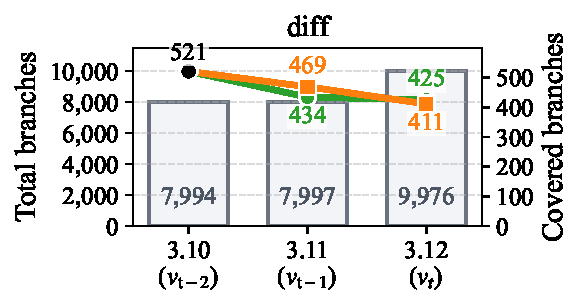
\includegraphics[clip, trim={0.25cm 0.3cm 0.35cm 0.25cm}, width=0.46\linewidth]{figures/fig_1_diff.pdf} &
        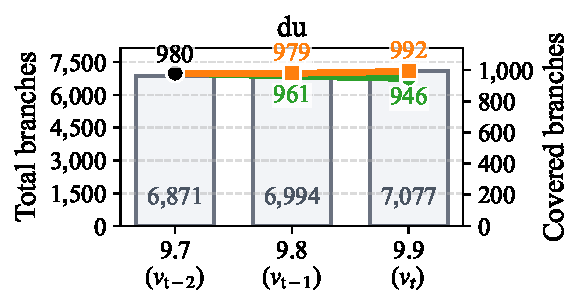
\includegraphics[clip, trim={0.25cm 0.3cm 0.35cm 0.25cm}, width=0.46\linewidth]{figures/fig_1_du.pdf} \\
        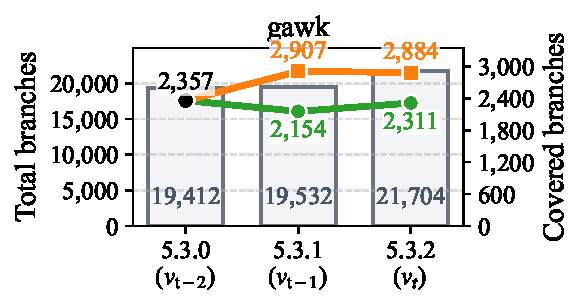
\includegraphics[clip, trim={0.25cm 0.3cm 0.35cm 0.25cm}, width=0.46\linewidth]{figures/fig_1_gawk.pdf} &
        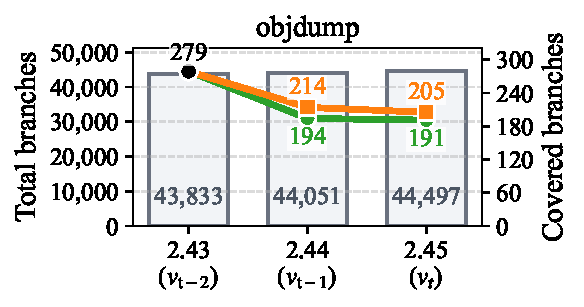
\includegraphics[clip, trim={0.25cm 0.3cm 0.35cm 0.25cm}, width=0.46\linewidth]{figures/fig_1_objdump.pdf} \\
        \multicolumn{2}{c}{
\includegraphics[clip, trim={0.0cm 0.25cm 0.0cm 0.18cm}, width=0.6\linewidth]{figures/fig_1_legend.pdf}}
    \end{tabular}
    \caption{Total branches and branch coverage across releases.}
    \label{fig:motivation}
\end{figure}

A key limitation of existing symbolic execution techniques is that they are not designed to exploit information accumulated across successive versions of the same program, despite the substantial overlap that typically exists between adjacent releases. As a result, they test each program version independently, repeatedly exploring similar program behaviors and solving similar constraints across successive versions. Consequently, they fail to improve their testing effectiveness even when programs evolve incrementally and information collected during prior testing runs could be reused.

To investigate the impact of this limitation, we ran a representative symbolic executor, KLEE~\cite{Cadar2008}, with a 12-hour testing budget on the latest three versions of four actively maintained GNU programs: \texttt{diff}, \texttt{du}, \texttt{gawk}, and \texttt{objdump}. For each program, we denote the latest version as $\newversion$, its immediately preceding version as $\prevversion$, and the version preceding that as $\prevtwoversion$. For each program version, we measured the number of branches covered by KLEE. 

Figure~\ref{fig:motivation} shows that KLEE typically fails to improve branch coverage across successive program versions. On average, the total number of branches increases by 5.1\% as new versions are released, whereas the number of branches covered by KLEE decreases by 7.0\%. This trend persists even though newer versions largely preserve existing code and introduce only incremental changes. Because KLEE tests each version from scratch, it cannot reuse information collected during previous test runs.

\begin{table}[]
    \centering
    \caption{Re-solving cost of recurrent path conditions across program versions.}
    \label{tab:redundant_queries}
    \resizebox{\columnwidth}{!}{
    \begin{tabular}{l||r|rr|rr}
    \toprule \midrule
    \multicolumn{1}{c||}{\multirow{2}{*}{\textbf{Program}}} & \multicolumn{1}{c|}{$\prevtwoversion$}    & \multicolumn{2}{c|}{$\prevversion$}                                            & \multicolumn{2}{c}{$\newversion$}                                                \\ \cmidrule(l){2-6}
    \multicolumn{1}{c||}{}                                  & \multicolumn{1}{c|}{\textbf{Solve Time(s)}} & \multicolumn{1}{c}{\textbf{Duplicate}} & \multicolumn{1}{c|}{\textbf{Re-solved(s)}} & \multicolumn{1}{c}{\textbf{Duplicate}} & \multicolumn{1}{c}{\textbf{Re-solved(s)}} \\ \midrule \midrule
    diff                                                   & 37,605.2                                    & 80.4\%                                 & 18,193.0                                   & 81.7\%                                 & 21,784.6                                  \\
    du                                                     & 41,793.1                                    & 94.9\%                                 & 41,884.1                                   & 96.0\%                                 & 42,490.8                                  \\
    gawk                                                   & 17,833.6                                    & 87.1\%                                 & 14,758.1                                   & 98.1\%                                 & 18,745.7                                  \\
    objdump                                                   & 41,474.8                                    & 96.9\%                                 & 37,424.0                                   & 99.8\%                                 & 37,833.6                                  \\ \midrule
    average                                                & 34,676.7                                    & 89.8\%                                 & 28,064.8                                   & 93.9\%                                 & 30,213.7                                  \\ \midrule \bottomrule
    \end{tabular}%
    }
\end{table}

A key reason for the limited effectiveness of symbolic execution on successive program versions is that a substantial portion of the testing budget is spent re-solving path conditions that were already solved during previous test runs. As shown in Table~\ref{tab:redundant_queries}, across the four programs, 89.8\% of the path conditions solved in $v_{t-1}$ had already been solved in $v_{t-2}$, consuming 7.8 hours (65.0\%) of the 12-hour testing budget. This redundancy becomes even more pronounced as programs continue to evolve. In $v_t$, 93.9\% of the solved path conditions had already appeared in either $v_{t-1}$ or $v_{t-2}$, and re-solving these recurrent path conditions consumed 8.4 hours (70.0\%) of the 12-hour testing budget. These results suggest that a large fraction of symbolic execution effort is repeatedly spent on previously explored execution paths rather than on newly introduced program behaviors.

